\documentclass[journal]{IEEEtran}
\usepackage[a5paper, margin=10mm, onecolumn]{geometry}
%\usepackage{lmodern} % Ensure lmodern is loaded for pdflatex
\usepackage{tfrupee} % Include tfrupee package

\setlength{\headheight}{1cm} % Set the height of the header box
\setlength{\headsep}{0mm}     % Set the distance between the header box and the top of the text

\usepackage{gvv-book}
\usepackage{gvv}
\usepackage{cite}
\usepackage{amsmath,amssymb,amsfonts,amsthm}
\usepackage{algorithmic}
\usepackage{graphicx}
\usepackage{textcomp}
\usepackage{xcolor}
\usepackage{txfonts}
\usepackage{listings}
\usepackage{enumitem}
\usepackage{mathtools}
\usepackage{gensymb}
\usepackage{comment}
\usepackage[breaklinks=true]{hyperref}
\usepackage{tkz-euclide} 
\usepackage{listings}
% \usepackage{gvv}                                        
\def\inputGnumericTable{}                                 
\usepackage[latin1]{inputenc}                                
\usepackage{color}                                            
\usepackage{array}                                            
\usepackage{longtable}                                       
\usepackage{calc}                                             
\usepackage{multirow}                                         
\usepackage{hhline}                                           
\usepackage{ifthen}                                           
\usepackage{lscape}
\begin{document}

\bibliographystyle{IEEEtran}
\vspace{3cm}

\title{10.3.2.2.1}
\author{EE24BTECH11064 - Harshil Rathan}
 \maketitle
% \newpage
% \bigskip
{\let\newpage\relax\maketitle}

\renewcommand{\thefigure}{\theenumi}
\renewcommand{\thetable}{\theenumi}
\setlength{\intextsep}{10pt} % Space between text and floats


\numberwithin{equation}{enumi}
\numberwithin{figure}{enumi}
\renewcommand{\thetable}{\theenumi}
\textbf{Question}:\\
On comparing the ratios $\frac{a_1}{a_2}$, $\frac{b_1}{b_2}$ and $\frac{c_1}{c_2}$ find out whether the lines representing the following pairs of linear equations intersect at a point, are parallel or coincident
\begin{align*}
    5x-4y+8 = 0 \\ 7x+6y-9 = 0 
\end{align*}
\\
\textbf{Solution: }\\
The general form of a pair of linear equations is given as:
\begin{align*}
    a_1x + b_1y + c_1 = 0, \\
    a_2x + b_2y + c_2 = 0.
\end{align*}
Here, the coefficients are:
\begin{align*}
    a_1 = 5, \quad b_1 = -4, \quad c_1 = 8, \\
    a_2 = 7, \quad b_2 = 6, \quad c_2 = -9.
\end{align*}
We calculate the ratios:
\begin{align*}
    \frac{a_1}{a_2} = \frac{5}{7}, \quad \frac{b_1}{b_2} = \frac{-4}{6} = \frac{-2}{3}, \quad \frac{c_1}{c_2} = \frac{8}{-9} = -\frac{8}{9}.
\end{align*}
Since $\frac{a_1}{a_2} \neq \frac{b_1}{b_2}$, the given lines intersect at a unique point.\\
\textbf{Solution using LU Decomposition}\\
Simplifying and using matrix notation,
\begin{align}
    5x-4y = -8\\
    7x+6y = 9 \\
    \myvec{
        5 & -4\\
        7 & 6
    } \myvec{x \\ y}= \myvec{ -8 \\ 9}
\end{align}

Any non-sigular matrix can be represented as a product of a lower triangular matrix $L$ and an
upper triangular matrix $U$

\begin{align}
    A\vec{x} = LU\vec{x} = \vec{b}
\end{align}
The upper triangular matrix U is found by row reducing A,
\begin{align}
    \myvec{5 & -4 \\ 7 & 6 } \xrightarrow{R_2 -> R_2 - \frac{7}{5}R_1} \myvec{5 & -4 \\ 0 & \frac{58}{5}}  
\end{align}
Let 
\begin{align}
    L = \myvec{1 & 0\\ l_{21} & 1}
\end{align}
$l_{21}$ is the multiplier used to zero $a_{21}$, so $l_{21} = \frac{7}{5}$.\\
\newline
Now,
\begin{align}
    A = \myvec{5 & -4 \\ 7 & 6} = \myvec{1 & 0 \\ \frac{7}{5} & 1}\myvec{5 & -4 \\ 0 & \frac{58}{5}}
\end{align}
Now we can get the solution to our problem by the two step process,
\begin{align}
    L\vec{y} = \vec{b}\\
    U\vec{x} = \vec{y}
\end{align}
Using forward substitution to solve the first equation,
\begin{align}
    \myvec{1 & 0 \\ \frac{7}{5} & 1}\myvec{y_1 \\ y_2} &= \myvec{-8 \\ 9}\\
    \xrightarrow{} \myvec{y_1 \\ y_2} &= \myvec{-8 \\ \frac{101}{5}} 
\end{align}
Now using back-substitution for the second equation,
\begin{align}
    \myvec{5 & -4 \\ 0 & \frac{58}{5}}\myvec{x_1 \\ x_2} &= \myvec{-8 \\ \frac{101}{5}}\\
    \myvec{x_1 \\ x_2} &= \myvec{\frac{-6}{29} \\ \frac{101}{58}}
\end{align}
The given pair of lines intersect at $\myvec{\frac{-6}{29} \\ \frac{101}{58}}$ and hence they are not parallel 
\begin{figure}[h!]
   \centering
   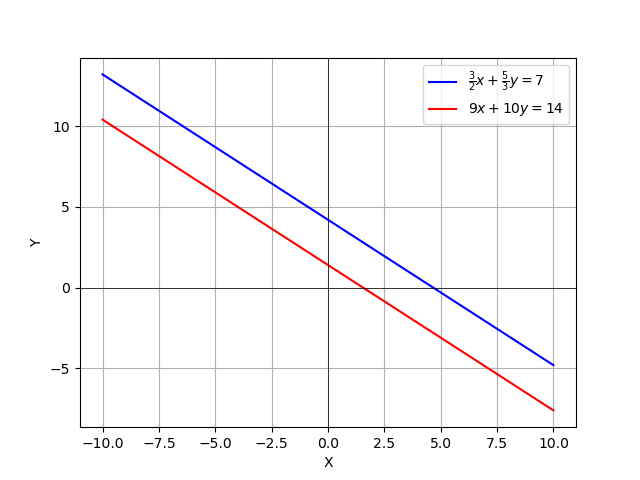
\includegraphics[width=\columnwidth]{figs/Figure_1.png}
\end{figure}
\end{document}
